
% this file is called up by thesis.tex
% content in this file will be fed into the main document

%: ----------------------- introduction file header -----------------------
\begin{savequote}[50mm]
Historical methodology, as I see it, is a product of common sense applied to circumstances. 
\qauthor{Samuel E. Morison}
\end{savequote}


\newcommand{\codigo}[1]{``\texttt{#1}''}
\newcommand{\primquery}{\emph{query}}
\newcommand{\primread}{\emph{read}}
\newcommand{\primtake}{\emph{take}}
\newcommand{\primwrite}{\emph{write}}


\chapter{Triple Space Computing for resource constrained devices}
\label{cha:tsc}
\newcommand{\pathchapthree}{3_tsc}

% the code below specifies where the figures are stored
\ifpdf
    \graphicspath{{\pathchapthree/figures/PNG/}{\pathchapthree/figures/PDF/}{\pathchapthree/figures/}}
\else
    \graphicspath{{\pathchapthree/figures/EPS/}{\pathchapthree/figures/}}
\fi



% ----------------------------------------------------------------------




Although in the Chapter~\ref{} and Chapter~\ref{} we refine how they work.
Particularly, 
regarding its network layer.
To make \ac{tsc}'s shared space over the network an underlying network-based architectural style needs to be chosen.


In recent years, the \acf{iot} has became a reality due to the increasing number of everyday objects with computing and networking capabilities.
The use of these everyday objects together with the rising of mobile computing greatly contributes to the \ac{ubicomp} vision.
In the beginning the community put more effort on those devices' connectivity issues, materialized in the spread of technologies such as Zigbee\footnote{http://www.zigbee.org}, 6LoWPAN\footnote{http://datatracker.ietf.org/wg/6lowpan/charter/} or Bluetooth\footnote{http://www.bluetooth.com}.
However, nowadays it is focusing on the architectural solutions used by the applications built around these objects.
A model to classify this solutions has been already presented in the previous chapter. % Coulouris et al.


% defendemos usar TSC
In this thesis, we defend that \acf{tsc} provides some valuable properties to \ac{ubicomp} environments. % mencionarlas?
However, some other properties are derived from how \ac{tsc} is implemented.
In this chapter we focus on selecting the underlying network-based architectural style.
% TODO problema: y por qué no otros? Habría que redactarlo de tal forma que no haga que un lector tiquismiquis requiera un puto survey de network-based architectural styles!
%This style guides how \ac{tsc}'s shared space is accessed over the network.
% In the Chapter~\ref{} and Chapter~\ref{} we define...


The REST architectural style, defended by the \acf{wot} initiative, is probably the most prominent architectural solution used for smart-objects. % probably porque no tengo datos que lo defiendan
The benefits that REST brings to resource constrained devices have been deeply described in the previous chapter.
However, in Section~\ref{} we analyze the characteristics of the style itself.

In Section~\ref{} we describe the similarities that \ac{tsc} has with the REST style.
Later, in Section~\ref{} we design a \ac{tsc} implementation which respects the REST principles.
The goal pursued is two-fold: (1) inherit most of the properties of REST and (2) maintain a high degree of compatibility with the \ac{wot}.
% on top of
% pros y contras

% Algunas ideas rescatables de la anterior intro:
% Both \ac{wot} and \ac{tsc} can be considered resource oriented solutions since they put emphasis in giving access to data resources.
% While \ac{tsc} enables expressive queries, dynamic discovery and non human-mediated cooperation among objects, the \ac{wot} adopts the scalable properties of the World Wide Web and it is entirely based on web standards.
% In this chapter we explain how to take advantage of both approaches, bringing together the best of both worlds.

% descripción de propiedades de REST: hipermedia distribuído
%    Requisitos de WWW: chapt4 de Fielding
%    network performance
%    UP performance
%    efficiency
%    scalability
%    simplicity
%    evolvability
%    extensibility
%    customization
%    configuration
%    reusability
%    visibility
%    portability
%    reliability
% Estilos de los que se deriva: ¿?
% descripción de requisitos REST: untangled
%    propiedades aportadas por REST a IoT
% Mención breve a HTTP y CoAP?

\section{\acl{rest}}

AA
% comparación de TSC y REST
%     id => XX
%   features añadidas por TSC (valuable properties aportadas)
%       utiles para IoT
%   cómo rompería alguna de las propiedades de REST
%   qué propiedades deseables para IoT añadiría TSC (per se)
% Ideas para citar:
%      TSC es como Web para semántica
%      RESTful semántico


\section{\acs{wot} and \acs{tsc} Comparison}
% 2. Comparativa
\label{sec:wot_tsc_comparison}

% TODO rehacer taaanto :-)

In this section, the strengths and weaknesses of both \ac{tsc} and REST approaches will be discussed and compared.
Then, their compatibility is shown by proposing two ways to use \ac{wot} solutions inside a \ac{tsc} environment and \textit{viceversa}.

The similarities and differences between \ac{wot} and \ac{tsc} which are summarized in the Table \ref{tab:comparison} are detailed below.

\begin{table}[ht!]
\centering
\caption {Comparison between \ac{wot} and \ac{tsc} (OtsoPack) resource-oriented approaches}
\begin{tabular}{|l|p{2,4cm}|p{2,6cm}|}
\hline
& \ac{wot} & \ac{tsc} (OtsoPack) \\
\hline
\textit{Architecture} & ROA \& C/S & ROA \& P2P \\
\textit{Communication} & HTTP & Jxta \\
\textit{Operations} & HTTP verbs & \ac{tsc} primitives \\
\textit{Format} & HTML, JSON \& XML & RDF (NTriples) \\ %content negotiation
\textit{Developer aid} & Less expressive data \& specific use & Expressiveness \& uniform API \\
\textit{Coupling} & Low & Very low \\ %data
\textit{Discovery} & Bad & Very good \\
\textit{Scalability} & Good & Bad \\
\textit{Semantics} & Microformats & Full \\
\hline
\end{tabular}
\label{tab:comparison}
\end{table}

\subsection{Architecture}
Both approaches are based on resource oriented architectures. \ac{wot} uses the REST architectural style, where the contents are directly addressable by
URLs to manipulate them, and \ac{tsc} creates, removes and modifies RDF triples or graphs, i.e. sets of interlinked triples, in a space formed by peers
in a P2P network.

Despite of these similarities, \ac{wot} uses a client-server architecture where each client has to know the URL where to address its operations, while
\ac{tsc} relies on a distributed shared memory which makes each process within a space completely autonomous. In \ac{tsc}, a node does not need to know where
information is stored, just the URI of the space it wants to query. Furthermore, the OtsoPack solution is fully distributed and conceived not to depend
on any centralized, previous known, intermediary server.

\subsection{Communication protocol}
Our \ac{tsc} solution currently uses Jxta\footnote{http://jxta.kenai.com/}, a language and platform independent \textit{Peer to Peer} protocol, to
interconnect the nodes and manage the groups (spaces) where they belong. Unfortunately, the mobile version relies in a Jxta gateway called Rendezvous
to propagate the messages to other nodes of the group, making some previous configuration necessary and potentially creating a bottleneck. Anyway,
some \ac{tsc} implementations such as TripCom\footnote{TripCom (IST-4-027324-STP, www.tripcom.org)} rely on HTTP, and one of our next steps will be the
reimplementation of our network communication through HTTP.

Even if it is not mandatory to comply with the RESTful style, \ac{wot} usually employs the HTTP protocol as a communication layer because of its
simplicity and wide adoption to ensure ample deployment.

\subsection{Operations}
\ac{wot} uses HTTP verbs to retrieve, create, modify or delete web resources. Retrieval is done using HTTP GET, creation by means of HTTP POST,
modifications with HTTP PUT and removals with HTTP DELETE. Finally, the HTTP OPTIONS command is used to introspectively find out what operations are
allowed for any URL.

\ac{tsc} and tuplespace solutions offer different primitives to write, read and delete content. In our solution, the previously explained \textit{write},
\textit{read} and \textit{take} primitives do that. Apart from these primitives, other ones are provided to manage spaces, to claim the manager role
for a type of content in a space, event notification or traditional request-reply style service consumption. Anyway, in this thesis we are going to focus in the
first ones because they are inherent to the \ac{tsc} paradigm. % innecesario mencionarlo?

\subsection{Format}
\ac{wot} usually returns a human readable HTML representation for a resource and XML or JSON common web representations to be used in mashups. One of the
key mechanisms that \ac{wot} inherits from HTTP is \textit{content negotiation}, which enables clients and servers to negotiate the requested and
provided representations for any given resource.

\ac{tsc} does not provide this response format negotiation mechanism. So, OtsoPack interchanges data in N-Triples format, which is the most primitive
representation of semantic data. In any case, other alternative semantic representations (e.g. RDF/XML, OWL/XML, Turtle or N3) could be
easily adopted as they basically describe the same RDF triples under different textual wrappers.

\subsection{Developer aid}%Actors}
In ROA an agreement about the data being exchanged and how it can be accessed is needed to develop applications.
On the one hand, \ac{wot} can define machine processable data using XML or JSON, but thanks to the Semantic Web \ac{tsc} can go one step
further formally defining them and making them also ``machine understandable'' (i.e. it is capable of inferring new knowledge and make
high-level queries over it).

On the other hand, both \ac{wot} and \ac{tsc} offer some operations and interfaces to access them. Whereas in \ac{tsc} this interface is the same in each node
and it is closely related with \ac{tsc} operations and resources, in \ac{wot} it changes in each application making a previous learning process necessary
to use them.

%Although applications which do not require human intervention can be built using RESTful services, one of the core concepts of \ac{wot} is the
%browse-ability of the object by the user using HTML. \ac{tsc} is a solution for the Semantic Web, which aims to provide a machine understandable
%web using ontologies and defining properties to enable inference.

\subsection{Coupling}
\label{sec:coupling}
The REST style describes loosely coupled services due to the platform independent, asynchronous and few self describing messages
\citep{pautasso_why_2009}. In a very similar manner, \ac{tsc} offers different kind of autonomies \citep{krummenacher_www_2005}:
\textit{time autonomy} (because of its asynchronous nature), \textit{location autonomy} (information providers and consumers are independent
from where the data is stored), \textit{reference autonomy} (nodes do not need to know each other) and
\textit{data schema autonomy} (it follows the RDF specification making it independent of nodes internal data schema).
% Quitado de la introducción para no repetirme
%Remarkably, \ac{tsc} guarantees four basic types of autonomies: \textit{space autonomy} (processes can be run in very different computational
%environments such as Android, Java ME devices or PCs, they just use a common coordination language), \textit{reference autonomy}
%(nodes do not need to know each other), \textit{time autonomy} (they communicate asynchronously) and \textit{data schema autonomy} (since
%written and read data is based on RDF triples, \ac{tsc} nodes are independent of their internal data schemas) \citep{fensel_triple-space_2004}.

In spite of the outlined decoupling nature of both approaches, the data definition can be considered a coupling mode indeed.
While in \ac{wot} each resource defines its own data formats and contents themselves, in \ac{tsc} the ontology in which the semantic
concepts are described must be known by each part of a distributed application to effectively cooperate among them.

\subsection{Discovery}
One of the main drawbacks in \ac{wot} is the lack of a discovery mechanism for new objects and the data they provide. Even when this data can be linked
in each object response (using HATEOAS) and microformats are sometimes included to ease the search-ability of these objects by search engines, it is difficult for an
object which may change of location and context to be referred. Thus, \ac{wot} may have a tendency to create isolated islands of data. Several workarounds
have been proposed to overcome this limitation, such as using a central repository\footnote{http://www.pachube.com/}, a framework which uses federated
repositories responsible for different administrative domains \citep{stirbu_towards_2008} or making each connected sensor announce itself to let an
intermediary know its presence \citep{kamilaris_smart_2010}.

\ac{tsc} provides a transparent data level discovery mechanism to the user since when a node joins a space (i.e. a group), its data become queriable by any other
node joint to this space. In OtsoPack the space management and communication relies on Jxta, a protocol which can be used at any level (even if we
have mainly used it on local environments using Jxta's discovery layer's capabilities).

\subsection{Scalability}
% TODO reescribir
The scalability of \ac{wot} is argued to be well proved since the World Wide Web is the most practical scalable system. As many objects as
necessary could be added to WWW without making it worse. 

Although Jxta scalability has been discussed and addressed in several works \citep{antoniu_performance_2007}, since our solution is fully decentralized
and uses flooding (each query is spread to the rest of the peers which belong to a space), its scalability is expected to be poor. To overcome this limitation,
we are working on implementing Semantic Overlay Networks (SON) to let the objects automatically divide the spaces into smaller ones and address queries
just to the appropriate nodes which conform a semantically related space.

% \begin{figure} [htbp]
% 	\centering
% 		\includegraphics[width=\linewidth]{./img/esquemaSON/arquitectura.png}
% 	\caption{Proposed distributed SON-based solution.}
% 	\label{fig:changeToSON}
% \end{figure}
% 
% As can be appreciated in Figure \ref{fig:changeToSON}, the proposed solution aims to split the spaces up into smaller subspaces.
% To do so, semantically similar contents are placed together in the same subspaces. E.g. \textit{subspaceA} contains \textit{graph1}
% and \textit{graph2} which describe ``light'' related knowledge. In the meantime, the nodes from the original space (\textit{space1}) can organize
% themselves to create another \textit{subspaceB} containing the relevant data for describing ``mobile phones''.

\subsection{Semantics}
On the one hand, \ac{wot} uses predefined microformats to embed semantic information into human readable pages. Doing so, the search process performed
by search engines is enhanced \citep{guinard_internet_2011}. On the other hand, \ac{tsc} allows the usage of full semantics, more expressive than microformats,
using RDF as a base. This makes \ac{tsc} capable of using standard query languages such as SPARQL and it becomes also independent of third parties' products to search data.



% 3. Ventajas ppales de cada uno
\subsection{Conclusion}
% TODO

In the previous section, the two-way compatibility between the \ac{tsc} and \ac{wot} approaches has been described. As has been shown, \ac{wot} is good due to its
scalability and usage of web standards, which makes it easy to be understood by potential developers (which encourages its usage). Our \ac{tsc}
solution, on the other hand, provides good local discovery of new resources and their information and allows more expressive semantic data
definition which leads to more expressive and sophisticated queries. Taking this into account, a scenario which takes advantage of the potential
combination of these approaches has been sketched (see Figure \ref{fig:scenario}).

% howto TSC over REST
% implementación: HTTP y porque no CoAP
% condiciones que hemos relajado de TSC (i.e. limitaciones)
%     1. autonomía espacial (dependes de un nodo)
%     2. consistencia de datos introducidos en el espacio
%     3. cómo asegurar un take?
%     4. subscripciones
%     + Hemos juntado como 2 mundos: TSC y WoT
%        La mayoría de las contribuciones son aplicables a WoT
%        El mecanismo de búsqueda no es Hypertext driven! (no?)
%        Por que sería muy costoso hacer rollo araña?!
%     5. Future work:
%          definir datos como consumibles por otros nodos o no
%          eliminar la necesidad de espacios?         
%     por qué creemos que sigue siendo útil?


% una comparación con nuestra solución propuesta
% cómo pueden interaccionar ambas
\section{First steps towards the integration of the \acs{wot} and \acs{tsc}}
% 2. Comparativa
\label{sec:integration_wot_tsc}

% TODO rehacer taaanto :-)


% existe gente que ha dicho que \ac{tsc} encaja con el pto de vista REST


% remarcar que en los primeros intentos se intentó esto, y luego lo otro

\subsection{Using \acs{wot} in a \acs{tsc} solution}
\label{sec:wotints}
To demonstrate the complete compatibility between \ac{tsc} and \ac{wot} approaches, we first used a \ac{wot} solution in a \ac{tsc} node. We used a gateway \cite{guinard_resource_2010} which provides access to sensors and actuators through RESTful services. To adapt it to the \ac{tsc} paradigm, we added to it a new data representation using a set of semantic triples (in this first approach, the solution is dependent on the ontology of the scenario).

In OtsoPack, each node is mainly made up of two parts: the network layer and the data access layer. While the first one has the responsibility of
keep a node communicated with the rest of the nodes of the space, the second one stores the triples managed by this node.
In OtsoSE we have replaced this data access layer to obtain the semantic information from the gateway instead of from a semantic repository.
Doing so, the \ac{tsc} primitives addressed to the gateway are translated into an HTTP request as summarized in Table \ref{tab:TS2WoT}.
\begin{table*}[t!] % http://en.wikibooks.org/wiki/LaTeX/Floats,_Figures_and_Captions#Wide_figures_in_two_column_documents
\centering
\caption {Mappings between OtsoPack's primitives and HTTP requests addressed to a \ac{wot} solution.}
\begin{tabular}{|c|p{10cm}|}
\hline
\acs{tsc} primitive & HTTP request \\
\hline \hline
read(spaceURI,[graphURI]) & HTTP GET over [graphURI] \\
\hline
read(spaceURI,[template]) & HTTP GET over http://gateway/read?template={''[template]``} \\
\hline
query(spaceURI,[template]) & HTTP GET over http://gateway/query?template={''[template]``}\\
\hline
write(spaceURI,[template]) & HTTP PUT over http://gateway/sunspots/[SpotName]/leds/led[0-6]

Parameters:
\begin{itemize}
  \item switch=[true/false]
  \item redColor=[0-255]
  \item blueColor=[0-255]
  \item greenColor=[0-255]
\end{itemize}

\\
\hline
\end{tabular}
\label{tab:TS2WoT}
\end{table*}

The Read primitive has two different types of implementations. In the most basic one, the graph is identified by a URI which in this case
coincides with the URL of the service that returns it (for example, in the case of temperature sensor
http://node/sunspots/\textit{SpotName}/sensors/temperature/). In the second implementation, the template is passed in as a query string parameter for
the GET command issued to a specific URL and the gateway checks all the graphs to facilitate a response. The Query operation has a similar behaviour.
The Write parses the contents of the triples extracting values and makes a POST request with them over a particular actuation service URL to change
its state.


% CONCLUSION: uso de gateways (a veces útil, pero no nuestro objetivo)


% mapping
% decir que ya hay muchos que intentaron esto antes: TSC?
\subsection{Making \acs{tsc} nodes part of the \acs{wot}}

\begin{table*}[t!] % http://en.wikibooks.org/wiki/LaTeX/Floats,_Figures_and_Captions#Wide_figures_in_two_column_documents
\centering
\caption {Examples of REST access to \ac{tsc} (\textit{sp:ex} is a space URI, \textit{sp:gr1} is a graph URI and templates are expressed between quotes)}
\begin{tabular}{|c|l|l|}
\hline
HTTP request & URL & Returns \\
\hline \hline
GET & http://nodeuri/prefixes & The list of prefixes used by the node \\
GET & http://nodeuri/prefixes/sp & The URI that ``sp'' prefix represents \\
POST & http://nodeuri/prefixes & Add a new prefix \\
 & \hspace{0.5cm}(parameters: \textit{URI} \& \textit{prefix name}) & \\
GET & http://nodeuri/sp:ex/query/any & \texttt{query(sp:ex,"?s ?p ?o ."): triples} \\
POST & http://nodeuri/sp:ex/graphs & \texttt{write(sp:ex,triples): URI} \\
 & \hspace{0.5cm}(parameter: \textit{triples}) & \\
GET & http://nodeuri/sp:ex/graphs & The list of graphs stored in this node \\
GET & http://nodeuri/sp:ex/graphs/sp:gr1 & \texttt{read(sp:ex,sp:gr1): triples} \\
GET & http://nodeuri/sp:ex/graphs/subject/sp:s1 & \texttt{read(sp:ex,"<sp:s1> ?p ?o ."): triples} \\
DELETE & http://nodeuri/sp:ex/graphs/sp:gr1 & \texttt{take(sp:ex,sp:gr1): triples} \\
DELETE & http://nodeuri/sp:ex/graphs/object/sp:o1 & \texttt{take(sp:ex,"?s ?p <sp:o1> ."): triples} \\
%GET & http://nodeuri/spaceuri/ontologies & The list of base ontologies used by the node \\
%GET & http://nodeuri/spaceuri/ontologies/rdfs & The triples which define RDF-Schema. \\
\hline
\end{tabular}
\label{tab:WoT2TS}
\end{table*}

In this section, a proposal to make any \ac{tsc} node \ac{wot} compliant is explained. To do that access to a \ac{tsc} should be provided through a RESTful service
(as shown in Table \ref{tab:WoT2TS}). As in \ac{tsc}, spaces, graphs, subjects, predicates and objects are identified by URIs, in order not to make the
requesting URLs too long, each node should provide a prefix mechanism to enable the URI shortening at \textit{http://nodeuri/prefixes/}.
This node will return all the prefixes used by this node, so they can be used inside any URL by simply using a name followed by '':`` and the last part of the URI.

To see the graphs available in a concrete node, \linebreak \textit{http://nodeuri/spaceuri/[graphs]} could be accessed. To access each graph
in a space, no matter if it is stored by the node responding to the HTTP request or not, we could access \textit{http://nodeuri/spaceuri/graphs/[graphuri]}.
It will be internally translated into a \primread primitive. To locate a graph giving a \textit{template} the accessed URL will be \linebreak
\textit{http://nodeuri/spaceuri/graphs/[template]}. The HTTP \linebreak DELETE verb should return the graph and delete it from the node where it was stored.

We propose specifying first a subject \textit{subject/[subj-uri]/} and concatenate \textit{/predicate/[pred-uri]/} and \textit{object/[obj-val]}\linebreak if needed to specify a \textit{template}. The order should be this, but any of them could be optional to express that any value could be ok (wildcard option). To express a \textit{?s ?p ?o .}-like template (any triple matches it), the URL ended by \textit{any} could be used.

To perform a \primquery \textit{http://node/spaceuri/query/[template]}-like URL should be accessed and to write a new graph the user should make a HTTP POST request to \linebreak \textit{http://nodeuri/spaceuri/graphs/} obtaining the new graph's URI as response.
%Additionally, some shortcuts could be proposed to explore the instance URIs of a given class (i.e. \linebreak 
%\textit{http://nodeuri/spaceuri/[classname]} would redirect to \linebreak \textit{http://nodeuri/spaceuri/query/p/rdf:type/o/[classname]}
%\footnote{For the sake of space ``predicate'' and ``object'' are represented by ``p'' and ``o''.}) \linebreak and an special URL to access to the base
\section{Refining integration} % repensar título y demás
% SECCIÓN: CUÁL ES EL DISEÑO GENERAL QUE SE PODRÍA UTILIZAR DESDE FUERA Y QUE HA MOTIVADO NUESTRA IMPLEMENTACIÓN
\section{Designing Triple Spaces over a canonical RESTful interface}
% ALGO QUE DIGA QUE NO DEPENDE DE OTSOPACK
% TODO: other name? ``defined layers'' o así? cómo decir ``mira, lo importante es que puede haber diferentes grados de
% implementación aquí gracias al diseño que mostramos en esta sección en 5 palabras???

So far, the compatibility of Triple Spaces with the HTTP RESTful style has been proved both from a formal \cite{hernandez_formal_2010} and qualitative point of view \cite{gomez-goiri_complementarity_2011}.
In this section our model towards the achievement of this mapping will be discussed in detail.

\subsection{TSC resources}

As was previously stated, our RESTful API is based on the Triple Space Computing paradigm, which is a Tuplespace variation where the information is stored in RDF.
Three key concepts are important at this point: agents share information in a common \textbf{space}.
A space is identified by an URI.
Therefore, all the operations performed in Triple Space are performed against a particular space.
By default, all applications should connect to a common standard space, but they can optionally choose to connect to a particular private space.
Within a space, the information is stored in sets of \textbf{triples} called \textbf{graphs}.
Each graph can also be identified by an URI. The RDF \textbf{triples} are the underlying concept of all the Semantic Web languages.
Each triple is composed by a subject (which is a URI), a predicate (also a URI) and a value (which can be a URI or a literal), as shown in the Figure \ref{fig:ontology}.

As detailed later, the operations supported by Otsopack attempt to add or remove graphs, as well as to query for graphs or query for sets of triples retrieved from different graphs.
In order to perform the queries, which enable the selection of a subset of the semantic content hold in a given space, a \textbf{template} is required.
Although more sophisticated query languages like SPARQL exist, in Otsopack wildcard templates are used, which are special triples with optional wildcard subject, predicate and/or objects.
For example, the template \texttt{?s foaf:knows kth:sven} could be employed to select instances which represent people who know Sven (see Figure \ref{fig:ontology}).


\InsertFig{semanticExample}{fig:ontology}{
  Semantic example
}{
  Sample triples expressed both grafically and in the RDF triple form.
  At the bottom a template example is shown.
  Aliases for the beginning of most URIs, known as prefixes in most Semantic languages, are used for the lack of clarity.
}{1}{}


\subsection{Adopted TSC primitives}
\label{sec:primitives}

TSC derives some primitives originally defined in the Linda language \cite{gelernter_generative_1985} to access to the semantic information hold in each graph.
In this section, these primitives will be explained.

\begin{itemize}
 \item The \textbf{write} primitive allows writing a graph into a given space (identified by its URI). The set of
triples received by this primitive will be stored together in the same graph, returning the URI which identifies that
graph. The graph URI can be used to access directly to that graph later on, or to create new triples and relate
contents.

  \begin{lstlisting}
    write(space_URI, triples): URI                [1]
  \end{lstlisting}


  \item The \textbf{read} returns a graph belonging to a given space which contains at least a triple matching the given
template or has the given URI as its identifier. If more than one graph fulfill one of these conditions, just one of
them is returned (nondeterministically). It should be remarked that it has been designed as a non blocking operation.
% why?
  \item The \textbf{take} primitive behaves like a destructive \textbf{read}, deleting the graph returned from the
space.

  \begin{lstlisting}
    read(space_URI, graph_URI): triples           [2]
    read(space_URI, template): triples            [3]
    take(space_URI, graph_URI): triples           [4]
    take(space_URI, template): triples            [5]
  \end{lstlisting}


  \item The \textbf{query} primitive aims to see the space as a whole triplestore, returning all the triples matching
the given template.
  \begin{lstlisting}
    query(space_URI,template): triples            [6]
  \end{lstlisting}

  \item Space management primitives. A node can join or leave a space using \linebreak \texttt{joinSpace(space\_URI)} or
\texttt{leaveSpace(space\_URI)}.
\end{itemize}



\subsection{HTTP API for TSC}
In the same way TSC has the explained primitives, HTTP has verbs to get, create, update or remove resources (GET,
PUT, POST, DELETE). Although the main purpose of TSC primitives is not the access to the data but the coordination of
the nodes accessing to that data, as both the RESTful style and TSC are resource oriented architectures, the translation
between these two worlds is straightforward (see Table \ref{tab:otsopackAPI}).


\begin{table} %http://en.wikibooks.org/wiki/LaTeX/Floats,_Figures_and_Captions#Wide_figures_in_two_column_documents
\centering
\caption {HTTP mapping for the primitives detailed in the section \ref{sec:primitives}. \textit{sp} is a
space URI, \textit{g} is a graph URI, \textit{s}, \textit{p} and \textit{o-uri} are subject, predicate and object URIs
or wildcards (represented with an as \textit{*}). When the template's object is a literal, it can be expressed
specifying its value (\textit{o-val}) and its type (\textit{o-type}).}
\begin{tabular}{|c|l|c|}
\hline
HTTP request & URL & Returns \\
\hline \hline
GET & \{sp\}/query/wildcards/\{s\}/\{p\}/\{o-uri\} &  [6] \\
 & \{sp\}/query/wildcards/\{s\}/\{p\}/\{o-type\}/\{o-val\} & \\
GET & \{sp\}/graphs/\{g\} & [2] \\
GET & \{sp\}/graphs/wildcards/\{s\}/\{p\}/\{o-uri\} & [3] \\
 & \{sp\}/graphs/wildcards/\{s\}/\{p\}/\{o-type\}/\{o-val\} & \\
DELETE & \{sp\}/graphs/\{g\} & [4] \\
DELETE & \{sp\}/graphs/wildcards/\{s\}/\{p\}/\{o-uri\} & [5] \\
 & \{sp\}/graphs/wildcards/\{s\}/\{p\}/\{o-type\}/\{o-val\} & \\
% ver como poner esto en una sola línea: As in our solution writings are made locally, POST is not mapped with
% write primitive} \\
\hline
\end{tabular}
\label{tab:otsopackAPI}
\end{table}

% Lo que quiero (yo Pablo) decir aquí es que sigue siendo distribuído aunque parezca que es uno a uno.

\subsubsection{Distribution}

The HTTP mapping presented is done among a \textit{client} and a \textit{server}.
However, as previously detailed, Triple Spaces provides reference autonomy, so a consumer will query the space without knowing the particular addresses of the nodes composing that space.
This autonomy is managed at other upper and optional layers explained in the following section, which manage the discovery.
However, this HTTP mapping is all a data provider needs to serve information in the space, and it is also what a data consumer needs to interrogate a multicast provider (a component provided by Otsopack to contact multiple nodes in a particular space).

\subsubsection{Status Codes}
Otsopack is compliant with the standardized HTTP status codes sent back as part of the header in the response (e.g. when no significant result can be found for a primitive the 404 error is returned).
This adoption - apart from enhancing the compatibility with other web applications - enables the modular adoption of our API and if a node does not offer a wildcard based \textit{query}, it will not affect the behavior of the rest of the nodes of an space.
Instead, they will interpret these cases as empty responses.
This modularity becomes crucial to ease the partial adoption on new platforms \cite{gomez-goiri_collaboration_2011}.

\subsection{Content Negotiation}
Another key aspect of the HTTP protocol we have taken advantage of is the \textit{content negotiation}.
This mechanism allows to specify the desired representation for a content on the client side and to express what representation is sent as a response from the data provider side.
For that purpose the client adds an \textit{Accept} field to the HTTP header with a weighted list of media types it understands and the server answers with the best possible format it knows about, specifying the \textit{Content-type} in the response.

In Otsopack this mechanisms not only enhance the browsability of the primitives with human understandable HTML responses, but they allows different Semantic representations (e.g. RDF/XML\footnote{http://www.w3.org/TR/REC-rdf-syntax/}, N-Triples\footnote{http://www.w3.org/2001/sw/RDFCore/ntriples/} or N3\footnote{http://www.w3.org/TeamSubmission/n3/}).
This characteristic becomes crucial since not all the nodes may understand all the languages (e.g. a mobile phone may not have a RDF/XML parser), even if they all use the same basic concepts: RDF Triples.
The compatibility of both sides can be ensured through a conversion carried out in the server side.
On the other hand, even if both the server and the client know how to use different languages, the preference of some of them can be easily expressed to achieve other goals (e.g. to obtain the less verbosed answer).


% SECCIÓN: CÓMO MOLA Y FUNCIONA NUESTRA IMPLEMENTACIÓN, QUE ES EL FOCO DEL PAPER
% 
% TODO: Poner que a pesar de que el ejemplo descrito no es real ha sido for the sake of clarity, pero 
% que el sistema ha sido utilizado en supermercados y hospitales reales como está descrito en [1] noticia en castellano [2] paper nuestro hablando de ello en otra confe pasada
% 
\section{Case study}

Otsopack has been used in real scenarios both in a supermarket and in a hospital with more complex applications within
the ACROSS project\footnote{\url{http://www.acrosspse.com/across/servlet/Noticias?id=33}\linebreak
\url{http://www.acrosspse.com/across/servlet/Noticias?id=35}}. For the sake of brevity and clarity, two simple and not
implemented applications have been designed for this contribution. The aim of them is to show how the middleware
solution can be used to achieve interoperability. In order to prove the feasibility of the implementation in limited
devices, times measured in real sensors are used.

For the case study, we will model two different applications: \textit{otsoSecurity} and \textit{otsoHomeAutomation},
which have not been implemented.

\subsection{Security}

A security company can develop an application which monitors different parameters such as the temperature, the humidity
or the $CO_2$ concentration with different sensors deployed over an industrial facility. Whenever any of this measures
go
beyond a determined threshold, the company needs to take the proper action. To answer to the potential risks the
application
creates tasks with different priorities: when a unimportant parameter is outside the expected boundaries the application
can write a low priority task for the security manager into the space (e.g. the $CO_2$ is slightly higher than the
normal one),
but to warn about an emergency to the users in the facility a high priority one can be written (e.g when they must leave
the building). Then, the message is consumed by different actuators according to its priority (e.g. in the manager's
phone in a less intrusive manner or through visual or auditory alarms over the building).

The company can also develop a simpler version of the same application for the workers' personal mobile phones to ensure
that they are warned even if the alarms of the main application fail. To implement both versions of the application,
commonly used ontologies such as SSN (Semantic Sensor Network Ontology) or SWEET (Semantic Web for Earth and
Environmental Terminology) can be used, storing and sharing the triples detailed in Listing~\ref{lst:security} in a
graph.

\begin{lstlisting}[label=lst:security,caption=Sample triples provided by a $NO_2$ sensor deployed in the facility.]

Subject       Predicate                Object

wot:meas1     rdf:type                 ssn:Observation
wot:meas1     ssn:observedProperty     sweet:NO2
wot:meas1     ssn:observationResult    wot:outpt1
wot:outpt1    ssn:hasValue             wot:val1
wot:val1      ssb:QuantityValue        17
wot:val1      dul:isClassifiedBy
                     muo-ucum:microgram-per-cubic-meter
...           ...                     ...
\end{lstlisting}


\subsection{Home automation}

On the one hand, a room has been populated with several kind of sensors connected to XBee sensors\footnote{\url{
http://tinyurl.com/xbee-sensors}} with an IP gateway\footnote{\url{http://tinyurl.com/connectportx2}},
FoxG20\footnote{\url{http://www.acmesystems.it}} embedded platform connected to sensors and to an actuator.
Besides, an Android application could be performed to semantically store the user's temperature preferences. An
independent
node (master node) continuously checks the room temperature using \textit{read primitive} to get the first available
graph
where the last measure is defined (no matter which device provides that information) and the user's desired temperature.
When the second one is below the first one, it generates a ``decrease temperature during a certain period'' task which
can
be consumed by different independent worker nodes. In this case, the FoxG20 periodically checks just for orders it can
fulfill and it understands and consumes them with a \textit{take primitive}.

Once again common ontologies such as SSN (Semantic Sensor Network Ontology), MUO (Measurement Units Ontology) or RECO
(RECommendations Ontology) are used to express these relations. Sample triples provided by the mobile phone can be found
in Listing~\ref{lst:home-automation}.

\begin{lstlisting}[label=lst:home-automation,caption=Sample triples stored by the Home Automation application.]

Subject       Predicate                Object

ud:aigomez    reco:desireTowards       ud:pref1
ud:pref1      rdf:type                 reco:Preference
ud:pref1      ssn:observedProperty     swt:Temperature
ud:prefm      ssn:observationResult    ud:dout1
ud:dout1      ssn:hasValue             ud:dVal
ud:dVal       ssn:QuantityValue        20
...           ...                      ...
\end{lstlisting}


\subsection{Interoperability}

\begin{sloppypar}
Given that both systems use a common ontology called SSN, and through Triple Spaces they can be using a common space,
whenever the Security application asks for triples matching a template \codigo{?s rdf:type sweet:Temperature}, the Home
automation application would return that \codigo{wot:mes3 rdf:type sweet:Temperature} along with other information
stored in that graph. Therefore, the Security application would be able to retrieve information from another application
it does not even know. In the same way, it is feasible that the Home automation application also retrieves information
stored by the Security application in the same or other nodes.
\end{sloppypar}

The key for this interoperability process is that both applications are using the same language, since both are using
the same concepts of the same ontologies (e.g. SSN). Although this can be achieved mapping concepts from two different
ontologies with a semantic web reasoner through the \codigo{owl:sameAs} property, it is habitual to use common
ontologies. Furthermore, since all the applications should be interested in retrieving data from other potential ones,
the developers should be willing to employ widely used ontologies to ease the information exchange among applications.

\subsection{Feasibility in embedded devices}

Finally, one of the challenges of Otsopack was to support limited devices such as low cost sensors. In order to do so,
two sensors are used: FoxG20\footnote{http://www.acmesystems.it} and XBee sensors with an IP
gateway\footnote{http://tinyurl.com/connectportx2gateways}. XBee can only be programmed in Python, so a subset of the
protocol was implemented in this language, only supporting that other nodes access sensor information in the space. 

Therefore, the rest of the nodes located in the shared space would be able to query the space and the sensors would
return the information. The requests performed by Android phones or PCs with Otsopack do not deal with the sensors in a
particular way, neither the Space Managers or other Otsopack components. They only query for certain information to the
space, and the sensors return the information if the query matches the information they contain.

To evaluate if this lightweight implementation of Otsopack fits, time measurements have been taken on both sensor
platforms under different levels of stress (from 1 concurrent request to 35), and they have been compared with a regular
PC running Otsopack (Java version), as shown in Figure \ref{fig:deviceComparison}. The results show that these sensors
can support a wide number of concurrent requests using this protocol, which should be enough in the described
scenarios. In any case, the design of the particular application should take into account the limits shown in the
figure.


% TODO: should we say something such as "the implementation required a few hundred lines of Python code" or so?
% Something to say "it was really small"

% \begin{figure}
% \centering
% 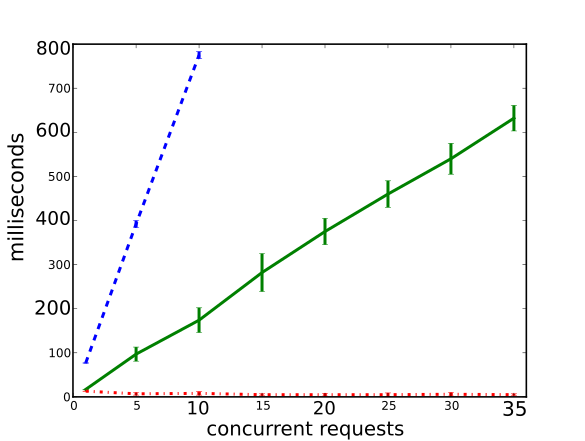
\includegraphics[width=3in]{images/device_comparison.png}
% \label{fig:deviceCompatison}
% \caption{Time measurement comparison among XBee sensors, FoxG20 and a regular computer}
% \end{figure}




\InsertFig{device_comparison}{fig:deviceComparison}{
  Response times measured in different embedded devices
}{
  The dash-dotted line represents the regular computer, the solid line the FoxG20 and the dashed line the XBee.
}{0.7}{}


\begin{table}[htbp]
    \caption{Mean of the measurements taken in different devices with the standard deviation ($\sigma$) in parenthesis.}
    \centering
    \begin{tabular}{|c|c|c|c|}
      \hline
      Concurrent & XBee & FoxG20 & Regular \\
      requests   &  & &  computer \\
      \hline
      1  &  77 (1)	&  17 (0)  &  13 (0) \\
      5  & 392 (8)	&  97 (16) &   7 (3) \\
      10 & 775 (8)	& 174 (28) &   8 (4) \\
      15 &  -	& 282 (43) &   5 (2) \\
      20 &  -	& 375 (30) &   5 (3) \\
      25 &  -	& 460 (30) &   5 (4) \\
      30 &  -	& 540 (35) &   6 (4) \\
      35 &  -	& 632 (29) &   5 (2) \\
      \hline
    \end{tabular}
    \label{tab:timeMeasures}
\end{table}
\section{Conclusion}
% 2. Comparativa
\label{sec:tsc_wot_conclusion}

% 5. otra forma de aunar las ventajas de ambos? => construir un TSC compatible con WoT (on top of that) <= integración profunda
%	Ventajas:
%		+ interoperable with other semantic WoT systems
%		+ syntactic services can still be provided using a different type of representation => WoT
%		+ promote indirect communication style => abstraction for the developer (does not care about manually discovering interfaces)
%	Problemas:
%		+ necesitas out-of-the-band conocimiento? API fija?
% esto trae problemas: cap 4 y cap 5


This chapter compares two different resource oriented approaches for the \acl{iot}: \acl{wot} and \acl{tsc}.
\ac{wot} seems to scale in a better way thanks to the underlying HTTP protocol, while \ac{tsc} performs the discovery process among locally available network-connected objects in a seamless way.
The first one is more human oriented and the second one relies on the Semantic Web capabilities to exchange a machine processable data.
Furthermore, the second one is ideal to easily configure intranets of network connected objects whilst the first one can easily bridge those intranets configuring global multi-site IoT ecosystems.

We deem that both approaches can win much from their combination since the weaknesses of one are outweighed by the strengths of the other.
Hence, they can be combined to offer a more scalable, machine and human processable solution that offers better cooperation possibilities among internet-connected objects and thus aid users in their daily activities.
As a simple proof of this hypothesis, a scenario employing \ac{wot} to export each space data to the outer world and \ac{tsc} to enable seamless and automatic configuration of heterogeneous devices on local networks has been presented.